\documentclass[a4paper]{article}
\usepackage[utf8]{inputenc}
\usepackage{graphicx}
\graphicspath{ {./images/} }
\usepackage{hyperref}
\hypersetup{
    colorlinks=true,
    urlcolor=blue,
    citecolor=black,
    }
\urlstyle{same}
\usepackage[fontsize=9pt]{fontsize}
\begin{document}

\title{COMP3100 project report}
\hrule \medskip
\begin{minipage}{0.9\textwidth}
\centering 
\large
Stage 2 COMP3100 Distributed Systems, S2, 2022\\
\normalsize
SID: 45334625, Name: Shakeel Mohammed
\end{minipage}
\medskip\hrule
\bigskip

\section{Introduction}
What is this project?
This report presented is to describe the overview, design, and implementation of a scheduling system that implements the Largest Round Robin algorithm whilst distributing jobs to servers in a simulated distributed system (provided by Macquarie University). The results generated by the use of this project are to be compared to a reference implementation (also provided by Macquarie University).

At it's core, a distributed system is a system that has various components which are spread across a network. This provides many advantages such as efficiency and redundancy, it also introduces complications such as an increased complexity, synchronisation and replication issues.

In a distributed system, the load is distributed across multiple machines to achieve fast and more reliable results. Each distributed system requires a component to orchestrate and distribute each request.

This project acts as an orchestrating component of a distributed system.

The goal for this project is to have a client which connects to the server, and makes scheduling decisions based on the desired algorithm.

\section{System Overview}
\label{sec:section2}
The system is comprised of two main components:
\begin{enumerate}
  \item The ds-sim Server - initiates the request to process each job, as well as simulates a distributed system.
  \item The Client (this project) - handles the request to process each job and schedules jobs for processing.
\end{enumerate}

\begin{center}
    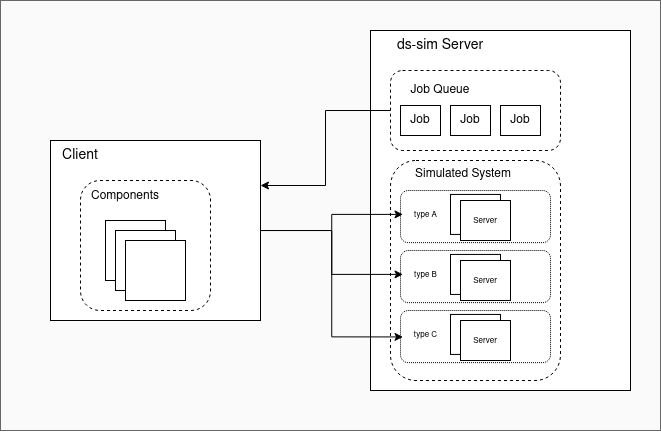
\includegraphics[scale=0.4]{images/ds-sim.png}
\end{center}

\subsection{Communication Protocol}
The two components communicate via a Socket. A socket is one endpoint of a two-way communication link between two programs running on the network \cite{sockets}.
The protocol is as follows:
\begin{enumerate}
  \item the ds-sim server is started, creates a simulated system based on the confile file passed in, and waits for incoming socket connections.
  \item the client is started and initiates a handshake with the server (client: HELO, server: OK, client: AUTH, server: OK).
  \item the server writes information on the simulated system to a ds-system.xml file.
  \item in a loop, the following happens:
  \begin{enumerate}
      \item the client sends REDY command.
      \item the server responds with either:
      \begin{enumerate}
          \item the server responds with JOBN (new job), and the client sends a SCHD command to schedule the job.
          \item the server responds with JCPL (completed), this is ignored.
          \item the server responds with an error, and the client logs the error and stops the job scheduling process.
          \item the server responds with NONE, this breaks the loop.
      \end{enumerate}
  \end{enumerate}
  \item once the loop is complete, the client sends QUIT command.
  \item the server replies with QUIT, and the connection is closed gracefully.
\end{enumerate}


\section{Design}
\label{sec:section3}
The design must cater for the connection between the two main components; the server and the client, as well as break down the current state of the simulated ds-sim system at any one time to handle incoming jobs. The two main entities in ds-sim are Servers and Jobs. These are the entities that are used to make scheduling decisions.

\subsection{Servers}
A server is a compute resource equipped with its own CPU, memory, and disk. They can be either physical or virtual servers. In the case of the ds-sim system, each simulated server is virtual. Each server has it's own serverId, serverType, limit, bootUpTime, hourlyRate, cores, memory, and disk attributes.

\subsection{Jobs}
A Job can represent a task, or a single linux process. Each job has it's own jobId, type, submitTime, estimatedRunTime, cores, memory, and disk attributes.

\subsection{Scheduling}
Processing information on each of these entities is crucial for our design to be able to achieve our goal to schedule jobs based on Largest Round Robin, which operates by scheduling jobs to servers that are of the type in the system have the highest number of cores, in a round robin manner. i.e. first job to server 1, second job to server 2, and so on.
\subsection{Components}
The design achieves job scheduling by Largest Round Robin by the use of the following components:

\subsubsection*{ConfigDataLoader}
A singleton object which serves as a configuration parameter store. It reads key/value pairs from the config.properties file. It allows the client to be re-configured without requiring re-compilation.

\subsubsection*{ClientServerConnection}
Handles the client/server socket connection. It provides an interface for the rest of the application to send and receive messages to the ds-sim server.

\subsubsection*{Orchestrator}
Responsible for making scheduling decisions. It currently implements the Largest Round Robin algorithm. It can easily be extended to support additional algorithms.

\subsubsection*{SimulatedSystem}
Responsible for containing information on the simulated system which the ds-sim server provides. It provides information on the system as a swarm of servers.

\subsubsection*{SimulatedServer}
Represents one server which exists in the ds-sim system. It contains information on the type of server, number of cores, etc.

\subsubsection*{Job}
Represents one job which exists in the ds-m system. It contains all of the attributes that define a job. A job is instantiated by the use of a JobInformation and a JobInformation component as they allow for a standardization layer. This is required because the ds-sim server is capable to providing a job in multiple different formats.

\subsection{Constraints}
This project requires a Java 1.8 to be run, which can be downloaded by following the instructions found
\href{https://docs.datastax.com/en/jdk-install/doc/jdk-install/installOpenJdkDeb.html}{here}.

\subsection{Considerations}
As per the ds-sim protocol, there are two methods by which a connecting client could retrieve information about the simulated system:
\begin{enumerate}
  \item ds-system.xml file - once the handshake is successful, the ds-sim server will create a ds-system.xml file which contains information on the simulated system in an xml format. This can then be parsed by the client.
  \item GETS command - a client is able to query the ds-sim server for a list of servers. This can be used to get a precise list of server capable of handing a job based on cpu, memory and disk, which are immediately available for use.
\end{enumerate}

This design uses option 2 to increase efficiency and search only for the servers that are capable of handling the particular job ready for processing. 


\section{Implementation}
\label{sec:section4}
\subsection{Technologies}
Java 1.8 - Java is a programming language and computing platform first released by Sun Microsystems in 1995. It has evolved from humble beginnings to power a large share of today’s digital world \cite{java}.

\subsection{Libraries}
The java client employs the use of the following classes provided by Java 1.8:
\begin{enumerate}
  \item Socket - A socket is an endpoint for communication between two machines. A socket is used for the client/server connection. The client/server connect via a Socket. This Socket connection is established and persisted throughout the entire run.
  \item DataInputStream - The client/server connection employs a DataInputStream to read responses from the server.
  \item File - The ConfigDataLoader employs the use of the java File class to create a File object, which represents the config.properties file. This object is then used to read each property.
  \item FileInputStream - The ConfigDataLoader employs the use of a FileInputStream to read each line from the config.properties file and store them.
  \item Properties - The ConfigDataLoader employs the user of a Properties object to presist the key/value pairs provided in the config.properties file.
  \item ArrayList - Java Arraylists are utilised by the SimulatedSystem class to keep track of the SimulatedServers within the system, as well as the SimulatedServer class to keep track of the Jobs relating to the SimulatedServer.
\end{enumerate}

\subsection{Job Scheduling}
The implementation as per the ds-sim protocol and Largest Round Robin is as follows:
\begin{enumerate}
    \item the main.java file initializes the Config Data Store and Client Server Connection. The client/server handshake process is handled.
    \item a new Orchestrator object is created with an empty SimulatedSystem and it's run() method is called.
    \item the Orchestrator object checks which algorithm it was configured with, and begins the largest round robin algorithm.
    \item in a loop, the following occurs:
    \begin{enumerate}
        \item the Orchestrator.runWithLargestRoundRobin() function issues a REDY command to the server.
        \item the server responds with either:
        \begin{enumerate}
            \item JOBN, where the Orchestrator builds a new Job object and uses the SimulatedSystem to query the server for servers capable of processing the job.
            \begin{enumerate}
                \item the server replies with the list of servers and the SimulatedSystem stores those servers.
                \item the Orchestrator uses SimulatedSystem.getTypeOfLargestServer, SimulatedSystem.findNextServerByType, and SimulatedServer.scheduleJob methods to find the largest type of server and get the next server based on the previously used server to schedule the job.
            \end{enumerate}
            \item JCPL, where the Orchestrator builds a new Job object and ignores the Job.
            \item NONE, where the loop is broken, the thread is returned back to the main.java file and the connection is ended gracefully
        \end{enumerate}
    \end{enumerate}
\end{enumerate}

\section{Usage}
\label{sec:section5}
\subsection{Compile}
A pre-compiled version of this project can be found in the /compiled directory. Otherwise, run "bash scripts/compile.bash" to compile the files in the /src directory and overwrite the files in the /compiled directory.

\subsection{Run}
Navigate to the config.properties file and observe the host IP, port, algorithm, are configurable from this file.
Navigate to the /compiled directory and run 'java Main'.

\section{GitHub Repository}
A link to the project GitHub repository can be found \href{https://github.com/shakeel-mohammed/client-server}{here}.
The privacy policy settings has been set to public to avoid any issues with access. The reference implementation can be found \href{https://github.com/distsys-MQ/ds-sim}{here}.

\bibliographystyle{plain}
\bibliography{bibliography.bib}

\end{document}
